\chapter{Conectividade e conjunto de dados}\label{cap:conectividade}
\rubricaJustificativa
\section{Tecnologia de comunicação}\label{sec:tecnologia}
O nó físico permaneceu num ambiente residencial de Teresina--PI com ponto de acesso doméstico à Internet por Wi-Fi 2,4~GHz; a distância real entre nó e roteador não foi medida. As mensagens de aproximadamente uma centena de bytes não exigem rádio de alta vazão, mas a aplicação precisa tanto enviar leituras periódicas como receber mudanças de configuração. O período da fase estável foi de 30~s (2.880 leituras/dia em operação contínua), e a coleta atravessou mais de um ciclo diurno/noturno. A decisão de comunicação foi quantitativamente motivada pela infraestrutura já disponível, não por uma avaliação fictícia de sinal RSSI.
\begin{table}[H]\centering\caption{Matriz de decisão de conectividade para a instalação observada}\label{tab:matriz}\scriptsize
\setlength{\tabcolsep}{3pt}
\begin{tabular}{@{}L{2.0cm}L{3.1cm}C{1.35cm}C{1.35cm}C{1.45cm}C{1.45cm}L{3.6cm}@{}}\toprule
\textbf{Critério}&\textbf{O que o projeto exige}&\textbf{Wi-Fi}&\textbf{BLE}&\textbf{LoRa/ LoRaWAN}&\textbf{NB-IoT/ LTE-M}&\textbf{Observação}\\\midrule
Alcance necessário&Mesmo cômodo do roteador doméstico; distância não aferida&\serve&\ressalva&\serve&\serve&BLE alcança poucos metros em ambiente interno e exige um central sempre ligado\\
Energia disponível&USB ou \emph{powerbank} de 10.000~mA\,h (Apêndice~\ref{ap:energia})&\ressalva&\serve&\serve&\ressalva&Na tomada não restringe; no \emph{powerbank}, o Wi-Fi é o maior consumo, não medido\\
Dado por transmissão&95 a 104 bytes de JSON a cada 30~s (2.880 mensagens/dia)&\serve&\serve&\naoserve&\serve&LoRaWAN: o JSON excede os 51 bytes do SF12 (AU915) e 2.880 mensagens/dia não cabem nos 30~s de ar por dia do TTN\\
Latência aceitável&Leitura em até um período (30~s); comando \texttt{config} aplicado na publicação seguinte&\serve&\serve&\ressalva&\serve&Mediana chegada$-$\texttt{ts} de 2,076~s (Tabela~\ref{tab:qualidade}); em LoRaWAN classe A o \emph{downlink} espera um \emph{uplink}\\
Infraestrutura no local&Wi-Fi 2,4~GHz e internet já existentes; nenhum \emph{gateway}, módulo LoRa ou chip celular&\serve&\naoserve&\naoserve&\naoserve&O kit não tem módulo LoRa nem modem celular; BLE precisaria de um \emph{gateway} para a internet\\
\bottomrule\end{tabular}\fonte{Elaborada pela equipe; as marcas de BLE, LoRaWAN e NB-IoT são avaliações técnicas, sem ensaio físico.}\end{table}
\begin{decisao}{Wi-Fi e MQTT 3.1.1 com EMQX Cloud}
\alternativas{Wi-Fi com MQTT, BLE mediante gateway, LoRaWAN mediante gateway e rede celular com modem.}
\criterio{Reaproveitar hardware e rede já presentes, permitir assinantes independentes e duas direções de mensagem sem gateway adicional.}
\escolha{Wi-Fi 2,4~GHz do ESP32; MQTT QoS 1 sobre o EMQX Cloud na porta 8883/TLS.}
\evidencia{3.082 telemetrias chegaram ao arquivo de disco, incluindo reconexões e comandos remotos; regularidade de 30~s no segmento de operação estável.}
\consequencia{Dependência de Wi-Fi e Internet; consumo do rádio não instrumentado; necessidade de gestão das credenciais e certificados. A escolha deixaria de valer se o nó fosse instalado fora do alcance do roteador (por exemplo, numa área externa da casa) ou tivesse de operar semanas só com bateria: nesse caso a leitura agregada, em formato binário de poucos bytes e com período de minutos, caberia em LoRaWAN, e um \emph{gateway} passaria a fazer parte do projeto.}
\end{decisao}
\section{Caminho do dado: do sensor ao CSV}\label{sec:caminho-dado}
O DHT11 é consultado a cada 2~s. A tarefa de telemetria incorpora a última medição em uma fila RAM de 120 entradas, atribuindo a cada registro a chave \texttt{(id, boot\_id, seq)} e um horário NTP quando válido. O cliente MQTT embarcado transmite \texttt{telemetria} para o EMQX. O broker distribui mensagens aos dois assinantes independentes: MQTTX para observação e \texttt{gravador.py} para persistência. O gravador Paho, em Windows, utiliza a sessão de identificador fixo e \texttt{manual\_ack=True}; escreve CSV com \texttt{flush()}, \texttt{fsync()} e posteriormente confirma o recebimento QoS~1. Falha de energia do nó destrói sua fila RAM, mas não apaga o contador persistido na NVS.\par
\begin{figure}[H]\centering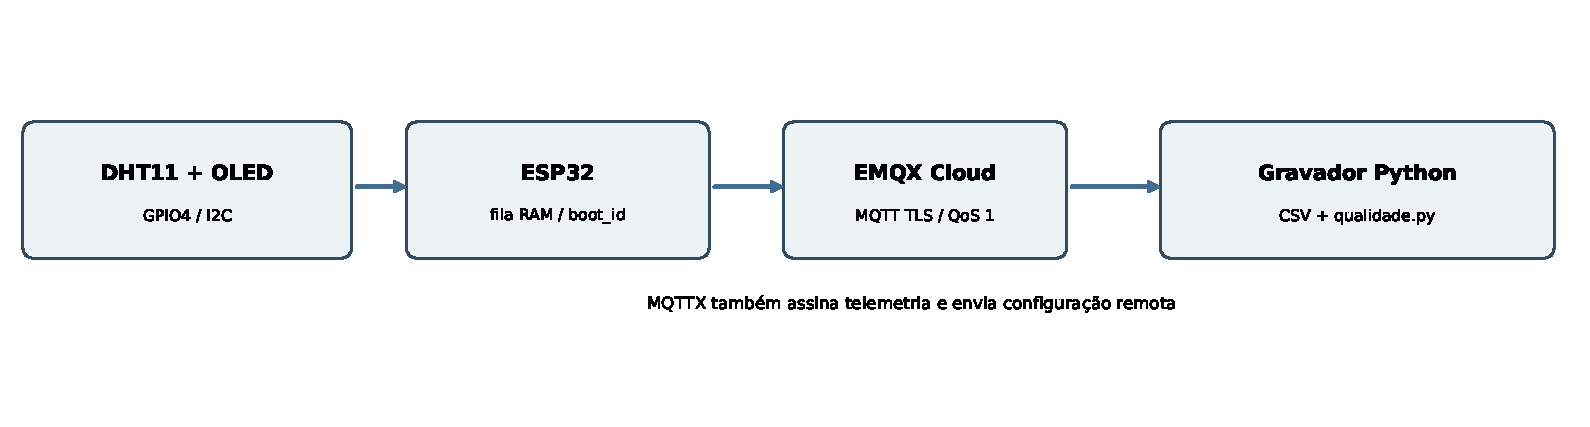
\includegraphics[width=.95\textwidth]{figuras/arquitetura.pdf}\caption{Caminho físico e lógico da aquisição ao arquivo CSV, utilizando EMQX Cloud.}\label{fig:caminho-final}\fonte{Equipe eq04.}\end{figure}
\begin{table}[H]\centering\caption{Onde roda cada peça, e o que acontece se ela parar}\label{tab:pecas}\footnotesize
\begin{tabular}{@{}L{3cm}L{5.3cm}L{5.5cm}@{}}\toprule
Componente&Papel na aplicação&Limite operacional\\\midrule
ESP32/DHT11/OLED&Aquisição, exibição, fila e publicação&Sem alimentação, não mede; fila é volátil\\
Wi-Fi local e Internet&Transporta pacotes MQTT/TLS ao broker&Leituras vão para a fila de 120 posições, que cobre 60~min a 30~s; na queda de 23/10 ela segurou 8 leituras\\
EMQX Cloud&Autenticação, autorização, roteamento, sessões, estado retido e LWT&Não substitui armazenamento histórico de dados\\
MQTTX&Recebe dados e publica configuração autorizada&Observação visual, não é gravador científico\\
Python/Paho e CSV, no notebook Windows 11 da residência&Grava mensagens com hora de recepção e metadados&Com sessão persistente o broker guarda as mensagens QoS~1 enquanto ele está parado (3 leituras na parada de 23/10, 14h38); o notebook precisa de internet, energia e disco\\\bottomrule\end{tabular}\fonte{Arquitetura efetivamente usada.}\end{table}
\section{Contrato de dados}\label{sec:contrato-dados}
A mensagem usa um contrato JSON explícito. A numeração \texttt{seq} reinicia após EN, enquanto \texttt{boot\_id}, armazenado na NVS com \texttt{Preferences}, identifica a inicialização. Assim duas mensagens com \texttt{seq=1} de inicializações distintas não representam a mesma leitura. O campo \texttt{ts} representa tempo de aquisição, não tempo de chegada ao notebook; pode valer \texttt{null} antes do ajuste de relógio NTP.
\begin{table}[H]\centering\caption{Campos e unidade do contrato publicado}\label{tab:contrato-dados}\footnotesize
\begin{tabular}{@{}L{2.15cm}L{1.55cm}L{1.9cm}L{3cm}L{4.5cm}@{}}\toprule
Campo&Tipo&Unidade&Exemplo real&Semântica\\\midrule
\texttt{id}&texto&---&\texttt{eq04-no02}&Nó de origem\\
\texttt{boot\_id}&inteiro&---&122&Inicialização NVS\\
\texttt{seq}&inteiro&---&25&Sequência da inicialização\\
\texttt{ts}&inteiro/null&Unix s&1792777341&Aquisição, após NTP\\
\texttt{sensor\_ok}&booleano&---&\texttt{true}&Leitura considerada válida\\
\texttt{temp\_c}&numérico/null&\si{\celsius}&36.3&Temperatura\\
\texttt{umid\_pct}&numérico/null&\%&37&Umidade relativa\\\bottomrule\end{tabular}\fonte{Payload real do CSV de 23/10.}\end{table}
\begin{lstlisting}[style=terminal,caption={Telemetria real com identificador de inicialização},label={lst:payload}]
{"id":"eq04-no02","boot_id":122,"seq":25,
 "ts":1792777341,"sensor_ok":true,
 "temp_c":36.3,"umid_pct":37}
\end{lstlisting}
A linha CSV adicional contém \texttt{t\_chegada}, \texttt{chegada} em ISO 8601, \texttt{topico}, \texttt{retido}, \texttt{payload}, \texttt{qos}, \texttt{dup}, \texttt{id}, \texttt{boot\_id} e \texttt{seq}. Os dois últimos são nulos para mensagens de estado ou configuração.\par
Esta é a versão do contrato que rodou na campanha (\texttt{firmware/higrolar\_ap2}). Ela difere do contrato-base da disciplina em dois pontos: a chave \texttt{boot} chama-se \texttt{boot\_id} e guarda um contador de inicializações na NVS, e a chave \texttt{sensor\_ok} foi acrescentada para que uma leitura inválida do DHT11 chegue ao arquivo marcada, com \texttt{temp\_c} e \texttt{umid\_pct} nulos, em vez de sumir. BLE foi descartado na Tabela~\ref{tab:matriz}; o projeto não usa contrato GATT.\par
\section{Contrato de tópicos, usuários e garantias}\label{sec:topicos}
O broker utilizado é \textbf{EMQX Cloud} (instância própria da equipe), em substituição à configuração HiveMQ do material de laboratório. A decisão foi operacional: utilizar um plano e instância que estavam acessíveis no período da atividade; não se afirma que todo plano HiveMQ seja pago, pois ofertas comerciais podem mudar. O endpoint pertence ao domínio \texttt{emqxsl.com}, na porta MQTT/TLS 8883. As telas de autenticação e autorização foram preservadas sem mostrar senhas.
\begin{table}[H]\centering\caption{Contrato de tópicos sob \texttt{ufpi-iot26/eq04/no02/}}\label{tab:topicos}\scriptsize
\setlength{\tabcolsep}{3pt}
\begin{tabular}{@{}L{1.8cm}L{2.3cm}C{0.7cm}C{1.3cm}L{2.4cm}L{5.7cm}@{}}\toprule
\textbf{Sufixo}&\textbf{Direção}&\textbf{QoS}&\textbf{Retido?}&\textbf{Quem assina}&\textbf{Por quê}\\\midrule
\texttt{telemetria}&nó $\to$ \emph{broker}&1&não&gravador e MQTTX&QoS~1 com sessão persistente não perde leitura com o gravador parado; a duplicata é descartada pelo \texttt{seq}. Sem retenção, um painel recém-aberto não mostra leitura velha como atual\\
\texttt{status}&nó $\to$ \emph{broker} (e testamento)&1&sim&gravador e MQTTX&Retido para que quem conecta saiba na hora se o nó está \texttt{online}; o testamento publica \texttt{offline} quando o nó cai sem avisar\\
\texttt{config}&MQTTX $\to$ \emph{broker} $\to$ nó&1&não&o nó&Muda o período sem regravar o firmware (\texttt{periodo\_s}: 30); QoS~1 porque um comando perdido deixaria o nó a 5~s\\
\bottomrule\end{tabular}\fonte{Elaborada pela equipe, a partir do contrato testado na campanha.}\end{table}
\noindent As quatro decisões que transformam um nó que publica num nó que forma um conjunto de dados:
\begin{description}[style=unboxed, leftmargin=0pt, font=\normalfont\bfseries]
  \item[1. Sessão persistente nos dois lados, com \emph{client ID} fixo.]\hfill\\
    O \emph{client ID} do nó é \texttt{ufpi-iot26-eq04-no02}; o do gravador, \texttt{ufpi-iot26-eq04-gravador}. Os dois conectam com \emph{clean session} desligada. Os IDs são distintos para que um cliente não derrube o outro. Quando o gravador parou às 14h38 de 23/10, o \emph{broker} guardou as leituras \texttt{seq} 16 a 18 do boot 122 e as entregou às 14h39min03s, com \texttt{session\_present} na reconexão.
  \item[2. O que o nó faz quando o \emph{broker} está fora de alcance.]\hfill\\
    A leitura é numerada e entra numa fila circular em RAM de 120 posições: 60~min a 30~s, ou 10~min a 5~s. Com a fila cheia, o firmware descarta a mais antiga e conta o descarte. Na queda de Wi-Fi de 23/10 a fila segurou 8 leituras (\texttt{seq} 14 a 21 do boot 121, carimbadas de 14h28min51s a 14h32min16s), entregues às 14h32min28s com o \texttt{ts} original. A fila não sobrevive a falta de energia.
  \item[3. \emph{Keepalive} e testamento.]\hfill\\
    \texttt{KEEPALIVE} de 30~s; pelo MQTT 3.1.1, o \emph{broker} declara o cliente morto depois de 1,5 $\times$ 30 = 45~s sem pacote e publica o testamento \texttt{offline}, retido. Na queda de 23/10, a última leitura entregue em tempo real foi a de 14h28min21s e a seguinte (14h28min51s) já foi para a fila; o \texttt{offline} apareceu às 14h29min16s, entre 25 e 55~s depois da perda, o que é compatível com o limite de 45~s. O laço não bloqueia além de \texttt{delay(1)}, bem abaixo desse limite.
  \item[4. Segurança mínima.]\hfill\\
    MQTT sobre TLS na porta 8883, com uma conta por papel no EMQX (Tabela~\ref{tab:contas}). As credenciais ficam em \texttt{secrets.h}, fora da árvore entregue, e o repositório traz só \texttt{secrets.example.h}. O gravador valida o certificado do servidor; o nó não, como descrito abaixo.
\end{description}
Foram cadastradas três identidades na autenticação MQTT do EMQX, com senhas separadas e \emph{client IDs} distintos. Elas cumprem papéis funcionais (não equivalem a permissões administrativas do painel). O modo de autorização exibido no EMQX é \emph{blacklist}, que permite solicitações não correspondentes a uma regra explícita; embora haja regras \emph{Allow} cadastradas, essa configuração \textbf{não implementa isolamento de acesso por padrão}. A mudança para \emph{whitelist} é recomendação de endurecimento para implantação posterior.
\begin{table}[H]\centering\caption{Contas do EMQX, papéis e permissões configuradas}\label{tab:contas}\scriptsize
\begin{tabular}{@{}L{2.5cm}L{2.55cm}L{4cm}L{5cm}@{}}\toprule
Usuário MQTT&Papel&Permissões exibidas&Uso no projeto\\\midrule
\texttt{higrolar-esp32}&Dispositivo&SUB \texttt{.../config}; PUB \texttt{.../status} e \texttt{.../telemetria}&Publicar leituras/estado; receber período\\
\texttt{higrolar-monitor}&Monitor e controle&SUB \texttt{ufpi-iot26/eq04/\#}; PUB \texttt{.../config}&Visualização MQTTX e comando remoto\\
\texttt{higrolar-gravador}&Coletor&SUB \texttt{ufpi-iot26/eq04/\#}&Paho, sessão persistente, escrita no CSV\\\bottomrule\end{tabular}\fonte{Capturas do painel EMQX na implantação eq04.}\end{table}
\begin{figure}[H]\centering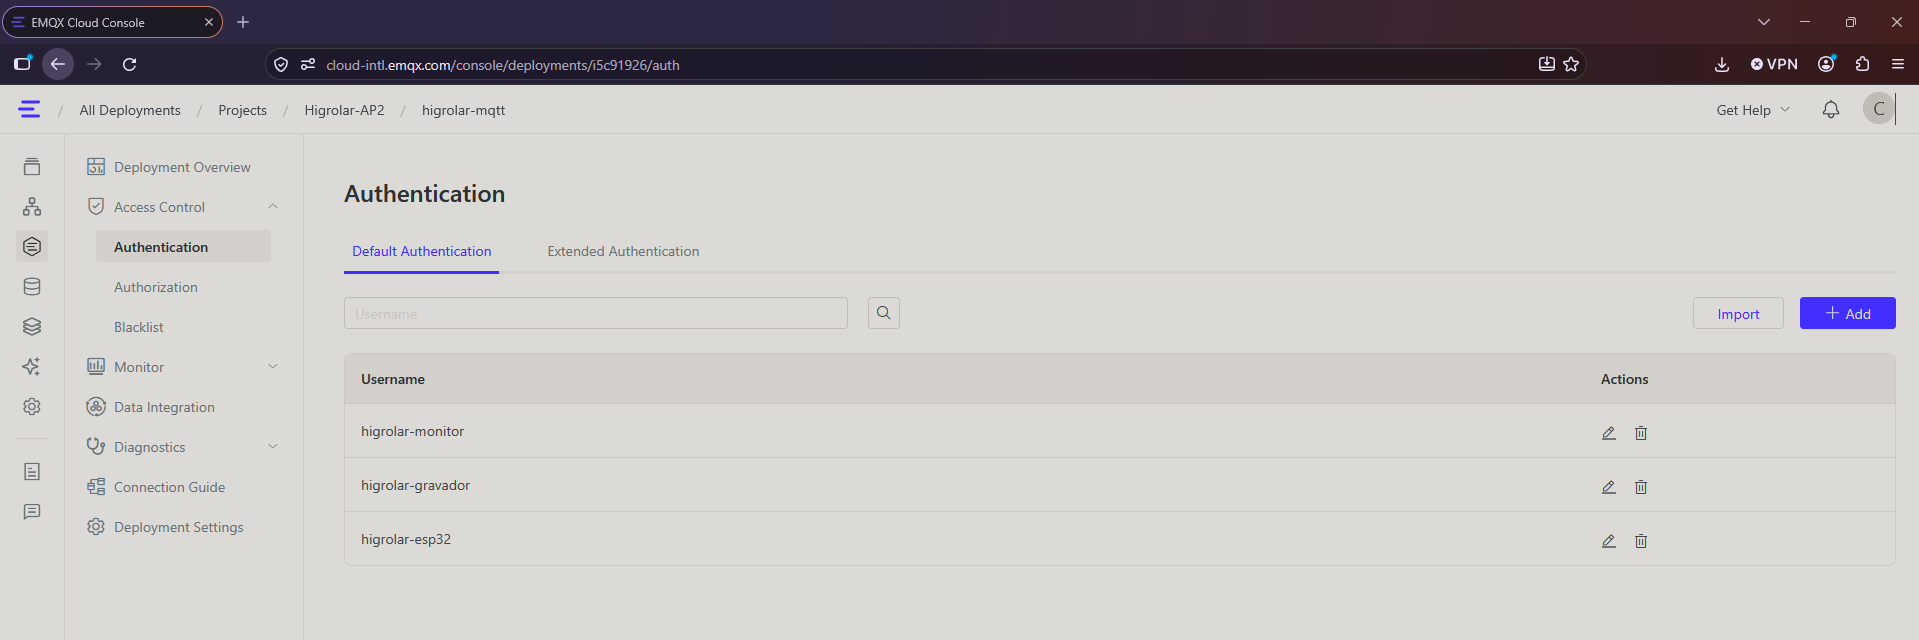
\includegraphics[width=.96\textwidth]{evidencias/prints/emqx_autenticacao.png}\caption{Contas MQTT separadas na autenticação do EMQX Cloud, sem exposição de senhas.}\label{fig:emqx-users}\fonte{Captura da equipe no console EMQX.}\end{figure}
\begin{figure}[H]\centering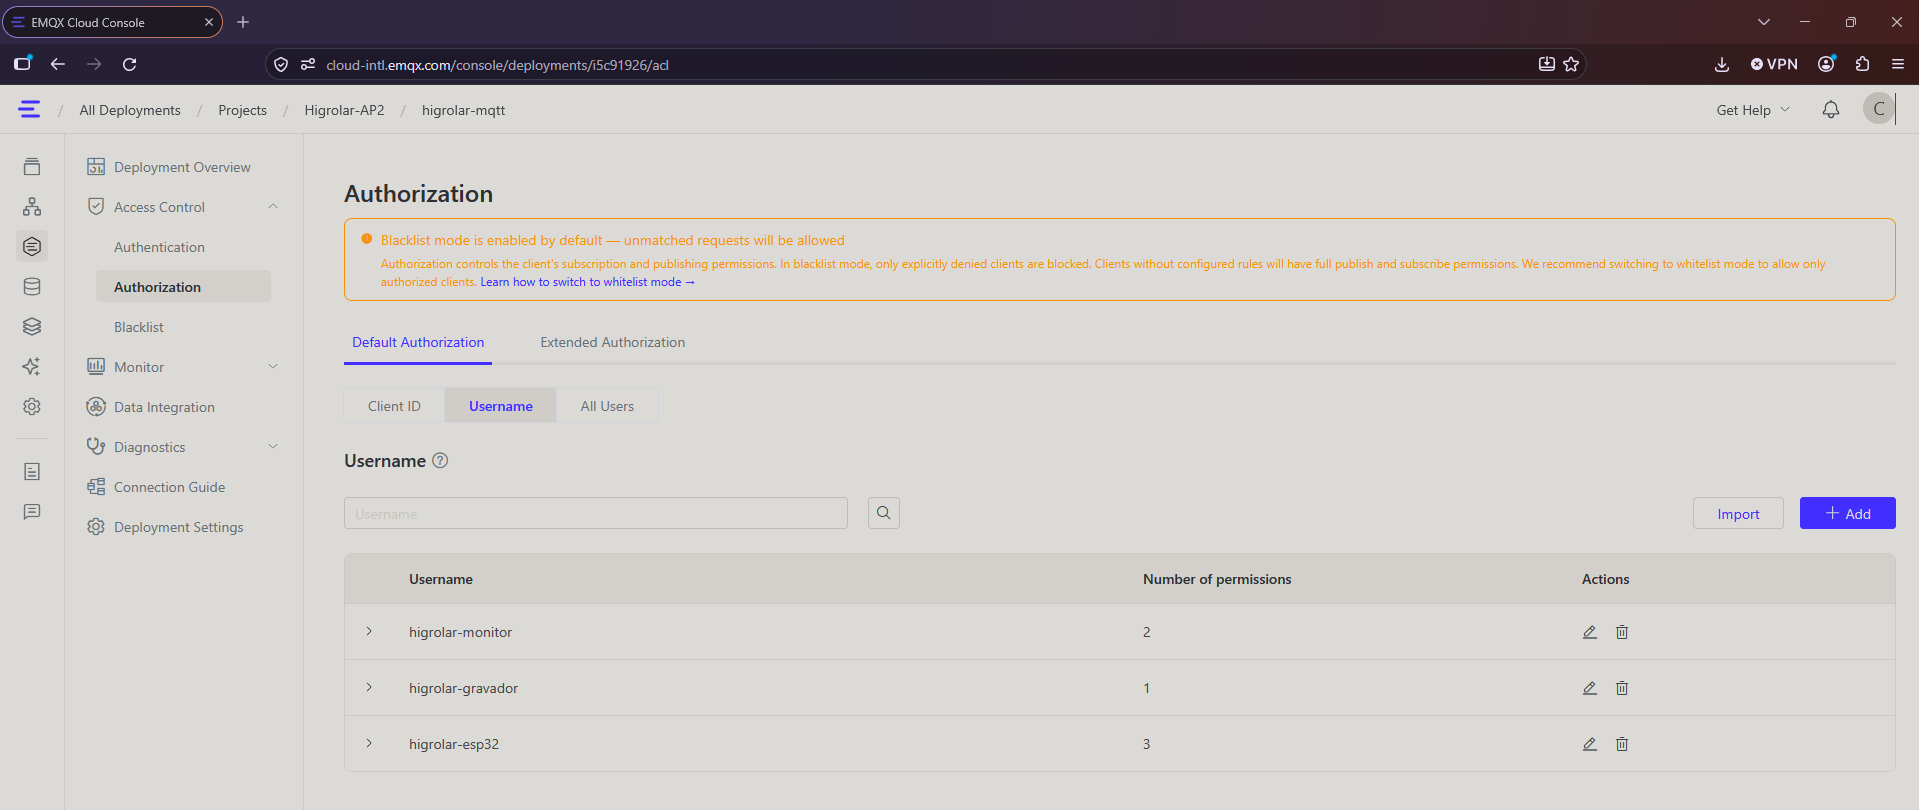
\includegraphics[width=.96\textwidth]{evidencias/prints/emqx_autorizacao.png}\caption{Modo de autorização \emph{blacklist} exibido no EMQX; solicitações sem regra explícita permanecem permitidas.}\label{fig:emqx-mode}\fonte{Captura da equipe no console EMQX.}\end{figure}
\begin{figure}[H]\centering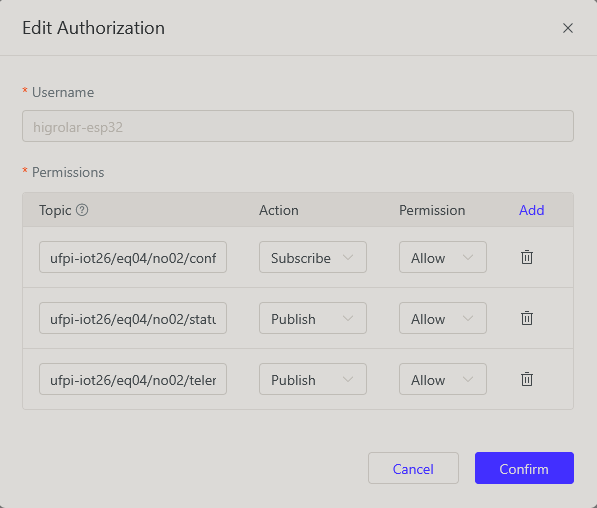
\includegraphics[width=.72\textwidth]{evidencias/prints/emqx_acl_esp32.png}\caption{Regras explícitas de \emph{publish/subscribe} cadastradas para o ESP32.}\label{fig:emqx-esp}\fonte{Captura da equipe.}\end{figure}
\begin{figure}[H]\centering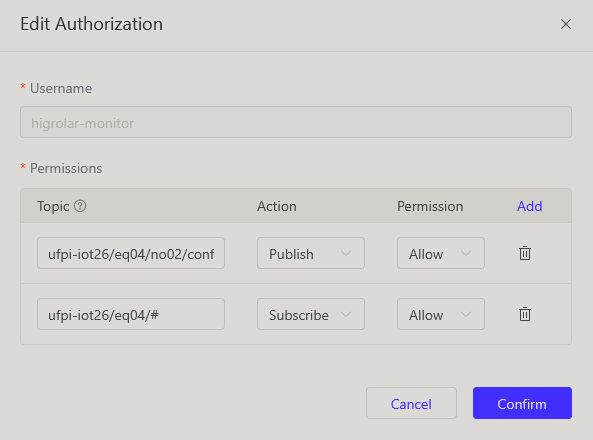
\includegraphics[width=.72\textwidth]{evidencias/prints/emqx_acl_monitor.png}\caption{Regras explícitas do monitor MQTTX: leitura da árvore e escrita em configuração.}\fonte{Captura da equipe.}\end{figure}
No cliente Python, a pilha SSL usa as autoridades certificadoras confiáveis do Windows e verifica a cadeia do servidor. No ESP32, o firmware usado na campanha chama \texttt{setInsecure()} na ausência de \texttt{MQTT\_CA\_PEM}; portanto o enlace é criptografado, mas \textbf{não valida a identidade remota} nessa configuração. Esta distinção é registrada como limitação de segurança, não ocultada pelo sucesso do MQTTX. O LWT \texttt{offline} é retido e publicado pelo broker quando a sessão falha. O QoS~1 permite entrega repetida; o identificador composto resolve duplicações lógicas no conjunto de dados, mas não evita mensagens não geradas ou perdas da fila volátil.\par
\section{Custo da comunicação}\label{sec:custo-radio}
A referência da AP1 era cerca de 75,4~mA de corrente média \emph{estimada}, anterior à ativação de Wi-Fi. A AP2 acrescentou associação, TLS, \emph{keepalive} e publicações de 30 em 30~s. A carga útil ideal de cerca de 100--140 bytes em 2.880 mensagens/dia corresponde a aproximadamente 0,29--0,40 MB/dia \emph{somente de payload}; o tráfego de rede real é maior. \textbf{A equipe não registrou corrente nem tempo do rádio com instrumento}; nenhuma autonomia com rádio é apresentada como medida.
\begin{table}[H]\centering\caption{Procedência do orçamento de energia}\label{tab:custo-radio}\footnotesize
\begin{tabular}{@{}L{4.5cm}L{3.1cm}L{6.5cm}@{}}\toprule
Item&Valor/estado&Origem e restrição\\\midrule
Corrente sem rádio&75,4 mA, estimativa&Orçamento anterior da AP1\\
Corrente rádio e duração de TLS&Não medidas&Requer medidor de corrente / \texttt{millis()}\\
Período de publicação estável&30 s&Comando MQTT e timestamp de aquisição\\
Autonomia real&Não determinada&Não extrapolar sem perfil de corrente\\\bottomrule\end{tabular}\fonte{Código, AP1 e dados da campanha.}\end{table}
O Apêndice~\ref{ap:energia} documenta cenários de sensibilidade; a ausência da medição de rádio permanece um requisito experimental não atendido.\par
\section{Campanha de coleta}\label{sec:campanha}
A campanha foi realizada no protótipo físico em ambiente residencial, com os equipamentos ambientais acionados manualmente e anotados no Apêndice~\ref{ap:campanha}. O intervalo entre a primeira e a última mensagem foi de \textbf{25h29min27s}, de 23/10/2026 às 14h27min27s a 24/10/2026 às 15h56min54s (UTC-3). O início contém os ensaios intencionais de falha e publicações com período de 5~s; a fase estável opera com período MQTT configurado em 30~s. Trata-se de uma janela suficiente para observar a alternância entre períodos diurno/noturno e múltiplas intervenções pontuais, mas não para demonstrar sazonalidade ou generalização.
\begin{table}[H]\centering\caption{Ficha final da campanha}\label{tab:campanha}\footnotesize
\begin{tabular}{@{}L{4.25cm}L{9.75cm}@{}}\toprule
Item&Valor efetivo e base de evidência\\\midrule
Local e nó&Ambiente residencial em Teresina--PI; \texttt{eq04-no02}, ESP32+DHT11+OLED\\
Broker&EMQX Cloud, MQTT 3.1.1, TLS na porta 8883\\
Recorte total&23/10 14h27min27s até 24/10 15h56min54s (UTC-3)\\
Duração do arquivo&25h29min27s\\
Volume MQTT&3.096 mensagens: 3.082 telemetrias, 12 estados e 2 configurações\\
Chaves únicas&3.080 telemetrias distintas por \texttt{(id,boot\_id,seq)}\\
Inicializações&\texttt{boot\_id}=120, 121, 122\\
Período&5~s inicial e 30~s após comando remoto, com interrupções deliberadas\\
Formato/arquivo&CSV bruto UTF-8, \texttt{dados/mensagens.csv}\\
Experimentos&Wi-Fi, reboot, gravador, NTP, umidificador, ar-condicionado, funcionamento conjunto\\
Período de amostragem&30~s; 5~s nos primeiros segundos de cada boot, até chegar o comando \texttt{config}\\
Janela do nó (primeiro e último \texttt{ts})&23/10 14h24min25s a 24/10 15h56min53s: 91.948~s\\
Leituras esperadas (duração $\div$ período)&3.080, somando os trechos da Tabela~\ref{tab:esperadas}\\
Número de nós&1 (\texttt{eq04-no02})\\
Onde rodou o gravador&Notebook com Windows 11 na mesma residência, ligado durante toda a coleta\\
Como a equipe acompanhou a coleta&\texttt{status} e telemetria no MQTTX; \texttt{qualidade.py} rodado durante a coleta (instantâneo de 24/10, 12h08, em \texttt{docs/evidencias/}) e sobre o arquivo final\\
Por que esta duração basta para a AP3&Cobre um ciclo dia--noite completo e oito intervalos de intervenção anotados (Tabela~\ref{tab:eventos}), o bastante para rótulos exploratórios. Não basta para generalizar: cada condição aconteceu uma ou duas vezes, num único cômodo e num único dia\\\bottomrule\end{tabular}\fonte{\texttt{mensagens.csv}, log final de qualidade e diário da equipe.}\end{table}
\noindent\textbf{Leituras esperadas.} A conta sai do tempo em que o nó deveria estar publicando dividido pelo período vigente em cada trecho, e não da contagem de linhas do arquivo. Como o período muda de 5 para 30~s dentro de cada boot, a conta é feita por trecho (Tabela~\ref{tab:esperadas}). Uma conta ingênua, com 30~s na janela inteira, daria $91.948/30 + 1 \approx 3.065$ leituras, menos do que as recebidas, porque ignora os trechos a 5~s. As leituras 1 a 18 do boot 120 não estão no arquivo, que começa na conexão do gravador de 23/10 às 14h27min27s, e ficam fora da conta.
\begin{table}[H]\centering\caption{Leituras esperadas por trecho da campanha}\label{tab:esperadas}\scriptsize
\begin{tabular}{@{}L{2.6cm}L{4.4cm}R{1.5cm}R{1.4cm}R{1.8cm}R{1.8cm}@{}}\toprule
\textbf{Trecho}&\textbf{Início -- fim (\texttt{ts} do nó)}&\textbf{Duração}&\textbf{Período}&\textbf{Esperadas}&\textbf{Únicas recebidas}\\\midrule
boot 120&23/10 14h24min25s -- 14h24min55s&30~s&30~s&2&2\\
boot 121, a 5~s&14h25min14s -- 14h25min51s&37~s&5~s&8&8\\
boot 121, a 30~s&14h25min51s -- 14h33min53s&482~s&30~s&16&16\\
boot 122, a 5~s&14h34min06s\textsuperscript{a} -- 14h34min51s&45~s&5~s&10&10\\
boot 122, a 30~s&14h34min51s -- 24/10 15h56min53s&91.322~s&30~s&3.044&3.044\\\midrule
\textbf{Total}&&&&\textbf{3.080}&\textbf{3.080}\\\bottomrule\end{tabular}\fonte{\texttt{dados/telemetria\_limpa.csv}. Esperadas $= 1 + \lfloor\text{duração}/\text{período}\rfloor$ no primeiro trecho de cada boot e $\lfloor\text{duração}/\text{período}\rfloor$ nos seguintes. \textsuperscript{a}Hora de chegada da leitura com \texttt{ts} nulo.}\end{table}
\section{Qualidade do conjunto de dados}\label{sec:qualidade}
O programa \texttt{qualidade.py} analisou exatamente o mesmo CSV final arquivado no projeto; sua saída completa encontra-se no Apêndice~\ref{ap:campanha}. Identificou 3.082 telemetrias recebidas, 3.080 únicas e duas repetidas pela chave composta; não encontrou saltos entre sequências mínimas e máximas dentro dos três \texttt{boot\_id} observados. Os três boots têm sequências 19--20, 1--24 e 1--3054, respectivamente. A completude de \textbf{100\%} relatada pelo programa é \textbf{interna aos intervalos numerados observados}; não se pode extrapolar automaticamente essa taxa para períodos sem numeração ou mensagens não criadas.
\begin{table}[H]\centering\caption{Indicadores de qualidade do CSV definitivo}\label{tab:qualidade}\footnotesize
\begin{tabular}{@{}L{7cm}R{3.2cm}L{3.1cm}@{}}\toprule
Indicador&Valor&Interpretação\\\midrule
Mensagens no arquivo&3.096&Conjunto final\\
Telemetrias recebidas&3.082&Inclui retransmissões\\
Telemetrias lógicas únicas&3.080&Chave por boot e seq\\
Duplicações lógicas&2&Retidas no CSV bruto\\
Saltos internos de sequência&0&Nos trechos observados\\
Fora de ordem&0&No log analisado\\
Boots observados&3&120, 121, 122\\
\texttt{ts} ausente&1&NTP ainda não válido\\
Falhas de sensor&0&Flag \texttt{sensor\_ok}\\
Atraso mediano (chegada--ts)&2,076~s&Depende dos relógios\\
P95 de chegada--ts&2,521~s&Desconsidera timestamp nulo\\
Máximo de chegada--ts&217,544~s&Inclui backlog intencional\\
Mensagens fora do contrato&0&Todas as 3.082 telemetrias têm as sete chaves da Tabela~\ref{tab:contrato-dados}\\\midrule
Leituras esperadas (conta)&3.080&Tabela~\ref{tab:esperadas}\\
\textbf{Completude}&\textbf{100\,\%}&3.080 únicas / 3.080 esperadas\\\bottomrule\end{tabular}\fonte{\texttt{qualidade.py}; saída literal no Apêndice F.}\end{table}
\noindent\textbf{Denominador da completude.} As leituras esperadas saem da conta da Tabela~\ref{tab:esperadas}, que usa a duração de cada trecho e o período vigente, e não o \texttt{seq}. As 3.080 leituras únicas cobrem as 3.080 esperadas. O resultado vale para a janela em que o nó estava ligado: o que ele não mediu enquanto reiniciava não existe no arquivo. Os dois reinícios duraram menos que um período de 30~s, então nenhuma leitura agendada se perdeu neles (Tabela~\ref{tab:lacunas}).\par
\begin{table}[H]\centering\caption{Lacunas e atrasos do conjunto de dados}\label{tab:lacunas}\scriptsize
\setlength{\tabcolsep}{3pt}
\begin{tabular}{@{}L{2.0cm}L{1.9cm}R{1.4cm}R{1.4cm}L{4.2cm}L{3.5cm}@{}}\toprule
\textbf{Início}&\textbf{Fim}&\textbf{Duração}&\textbf{Leituras perdidas}&\textbf{Causa}&\textbf{Tratamento}\\\midrule
23/10 14h24min55s&14h25min14s&19~s&0&Reinício 120 $\to$ 121, antes do início do diário; causa não anotada&Mantido; o \texttt{boot\_id} separa os trechos\\
23/10 14h28min51s&14h32min28s&217~s&0&Wi-Fi interrompido de propósito (\CT{03}); 8 leituras ficaram na fila do nó&Nenhum: chegaram atrasadas com o \texttt{ts} original\\
23/10 14h33min53s&14h34min06s&13~s&0&Botão EN (\CT{05})&Mantido; o \texttt{boot\_id} separa os trechos\\
23/10 14h37min51s&14h39min03s&72~s&0&Gravador parado de propósito (\CT{06}); 3 leituras guardadas pelo \emph{broker}&Nenhum: entregues na reconexão\\
23/10 14h42min22s&14h42min24s&2~s&0&\texttt{offline}/\texttt{online} transitório, causa não aferida; \texttt{seq} 25 chegou duas vezes&Duplicata descartada pela chave lógica\\
24/10 11h47min25s&11h47min26s&1~s&0&\texttt{offline}/\texttt{online} sem intervenção anotada; \texttt{seq} 2555 chegou duas vezes&Duplicata descartada pela chave lógica\\\bottomrule\end{tabular}\fonte{\texttt{dados/mensagens.csv} e \texttt{dados/telemetria\_limpa.csv}. Nenhum trecho foi interpolado.}\end{table}
\noindent\textbf{Interpretação de atraso.} O valor de \texttt{chegada-ts} mede a diferença entre relógios da estação e o timestamp embarcado, incluindo fila do broker, rede e backlog. Após o Wi-Fi retornar, diversos registros antigos chegam em poucos segundos, produzindo máximo de 217,544~s sem representar latência típica do enlace. O \texttt{DUP} MQTT permaneceu 0, o que não impede as duas repetições lógicas identificadas.\par
\section{Descrição do conjunto de dados}\label{sec:dataset}
O conjunto tem dois arquivos em \texttt{dados/}. O \textbf{bruto}, \texttt{mensagens.csv}, é a saída do gravador sem edição: 3.096 registros (3.082 telemetrias, 12 estados e 2 configurações), 680~kB, com dez colunas: \texttt{t\_chegada}, \texttt{chegada}, \texttt{topico}, \texttt{retido}, \texttt{payload}, \texttt{qos}, \texttt{dup}, \texttt{id}, \texttt{boot\_id} e \texttt{seq}. Ele guarda as duplicatas e as mensagens de estado como evidência. O \textbf{limpo}, \texttt{telemetria\_limpa.csv}, é gerado por \texttt{dados/limpar.py}: mantém só a telemetria, descarta as repetições pela chave \texttt{(id, boot\_id, seq)} e abre o JSON em colunas. São 3.080 linhas e 270~kB. Nenhum valor é interpolado ou preenchido; a Tabela~\ref{tab:dataset} descreve as colunas do arquivo limpo.\par
\begin{table}[H]\centering\caption{Descrição do conjunto de dados limpo}\label{tab:dataset}\scriptsize
\setlength{\tabcolsep}{3pt}
\begin{tabular}{@{}L{1.7cm}L{1.6cm}L{1.6cm}L{4.0cm}L{5.4cm}@{}}\toprule
\textbf{Campo}&\textbf{Tipo}&\textbf{Unidade}&\textbf{Faixa observada}&\textbf{Observação}\\\midrule
\texttt{id}&texto&---&\texttt{eq04-no02}&Um único nó\\
\texttt{boot\_id}&inteiro&---&120 a 122&Contador de inicializações na NVS\\
\texttt{seq}&inteiro&---&1 a 3.054&Reinicia a cada boot\\
\texttt{ts}&inteiro ou vazio&s (época Unix)&1792776265 a 1792868213 (23/10 14h24min25s a 24/10 15h56min53s)&Hora da última leitura do DHT11 antes da publicação; vazio em 1 linha (antes do NTP)\\
\texttt{ts\_local}&texto&ISO 8601, UTC-3&mesma janela de \texttt{ts}&\texttt{ts} convertido; na linha sem \texttt{ts}, a hora de chegada\\
\texttt{ts\_origem}&texto&---&\texttt{no} (3.079) ou \texttt{chegada} (1)&Diz de onde veio \texttt{ts\_local}\\
\texttt{t\_chegada}&real&s (época Unix)&1792776447,018 a 1792868214,495&Hora em que o gravador recebeu a mensagem\\
\texttt{sensor\_ok}&booleano&---&sempre \texttt{true}&Nenhuma falha de leitura na campanha\\
\texttt{temp\_c}&real&\si{\celsius}&26,9 a 36,9&Resolução de 0,1~\si{\celsius}\\
\texttt{umid\_pct}&inteiro&\% UR&34 a 73&Resolução de 1\,\%; 40 valores distintos\\\bottomrule\end{tabular}\fonte{\texttt{dados/telemetria\_limpa.csv}, gerado por \texttt{dados/limpar.py} a partir de \texttt{dados/mensagens.csv}.}\end{table}
\noindent Arquivos: \texttt{dados/mensagens.csv} (bruto) e \texttt{dados/telemetria\_limpa.csv} (limpo).\\ \emph{Commit}: o da \emph{tag} \texttt{ap2}; o bruto entrou no \texttt{e722db7} e não mudou depois.\par
Para a análise da série ambiental usa-se o arquivo limpo, ordenado por \texttt{ts\_local}. Temperatura e umidade relativa são medidas físicas do DHT11 num único ponto do cômodo.\par
\noindent\textbf{O que a equipe quer que um modelo aprenda com estes dados.} Reconhecer, pela forma das curvas de temperatura e umidade, em que condição o ambiente está: sem aparelhos, umidificador ligado, ar-condicionado ligado, os dois juntos ou janela aberta.\par
\noindent\textbf{O conjunto tem exemplos suficientes disso?} Para rótulos exploratórios, sim. Para treino supervisionado, ainda não. O registro de eventos (Tabela~\ref{tab:eventos}) dá oito intervalos com hora: umidificador sozinho duas vezes (23/10 15h33--18h43 e 24/10 12h03--12h59), ar sozinho duas vezes (24/10 01h05--04h05 e 14h10--15h02), os dois juntos duas vezes (12h59--14h10 e 15h02--15h19) e janela aberta duas vezes (com e sem umidificador). Com uma ou duas ocorrências por classe, num único cômodo e com um único sensor de baixa resolução, a AP3 precisa de novas campanhas em outros dias antes de treinar e avaliar um classificador.
